\documentclass[11pt]{article}
\usepackage[margin=1in]{geometry}
\usepackage{graphicx}
\usepackage{amsmath}
\usepackage{siunitx}
\usepackage{booktabs}
\usepackage{hyperref}
\usepackage{caption}
\usepackage{float}
\usepackage{setspace}
\setstretch{1.05}

\title{\textbf{Relationship Between Source Position and Absorber Thickness}\\
\textbf{Co-60 Gamma Attenuation with a Geiger--M\"uller Counter}}
\author{Hongyu Wang\\Department of Physics, University of California, Santa Barbara\\Instructor: W. Lippincott}
\date{June 5, 2024}

\begin{document}
\maketitle

\begin{abstract}
We quantify how a geometric change in source position alters the absorber thickness required to obtain a target \emph{net} count rate in a Co-60 attenuation experiment.
Using a Geiger--M\"uller (GM) counter and a set of calibrated absorbers (areal density $Z$ in \si{mg.cm^{-2}}), we measured background-subtracted count rates $(N-B)$ at multiple $Z$ values for different source slots.
Over the gamma-dominated regime ($Z\gtrsim\SI{3700}{mg.cm^{-2}}$), linear regression yields
$ (N-B) = (-8.57\times10^{-3})Z + 263.00$ for Slot~3 and $(N-B) = (-5.95\times10^{-3})Z + 177.95$ for Slot~4 (rates in \si{min^{-1}}).
Inverting these relations gives an empirical mapping between source displacement (Slot~4\,$\rightarrow$\,Slot~3, separation \SI{0.876}{cm}) and additional absorber thickness
$\Delta Z \approx 51.38\,(N-B) + 781$ \si{mg.cm^{-2}}.
For a representative operating point $(N-B)=130$ \si{min^{-1}}, moving the source from Slot~4 to Slot~3 requires an additional \SI{7.46e3}{mg.cm^{-2}} of absorber to match the same net rate.
A separate control study shows the absorber position (among adjacent slots) does not significantly change the net rate at fixed $Z$ (one-way ANOVA $p=0.70$).
\end{abstract}

\section{Objective and background}
Gamma-ray attenuation experiments often assume that count rate is determined primarily by absorber thickness.
In practice, the measurement geometry---especially source--detector distance---can introduce comparable changes through solid-angle effects and scattering.
This lab quantifies the coupling between \emph{source position} and \emph{absorber areal density} required to maintain a chosen net count rate.

Co-60 decays by $\beta^-$ emission to excited \mbox{Ni-60}, followed by two prompt gamma rays at approximately \SI{1.173}{MeV} and \SI{1.332}{MeV}.
At low absorber thickness, the GM tube can register both beta and gamma radiation; therefore, we restrict our regression analysis to a gamma-dominated thickness range (Sec.~\ref{sec:analysis}).

\section{Experimental setup}
\subsection{Apparatus}
Measurements used a Co-60 source, a GM counter operated at \SI{500}{V}, and a slot-based holder that allowed discrete changes in source position and absorber placement.
Absorbers were specified by their areal density $Z$ (\si{mg.cm^{-2}}).
Count rates were recorded in counts per minute (cpm).

\subsection{Slot spacing}
To document geometry, we measured the spacing between adjacent slots from a calibrated photograph using Fiji.
Five independent measurements produced an average separation of
\begin{equation}
\Delta x = \SI{0.876}{cm} \quad (\sigma\approx\SI{0.042}{cm}).
\end{equation}
\begin{figure}[H]
  \centering
  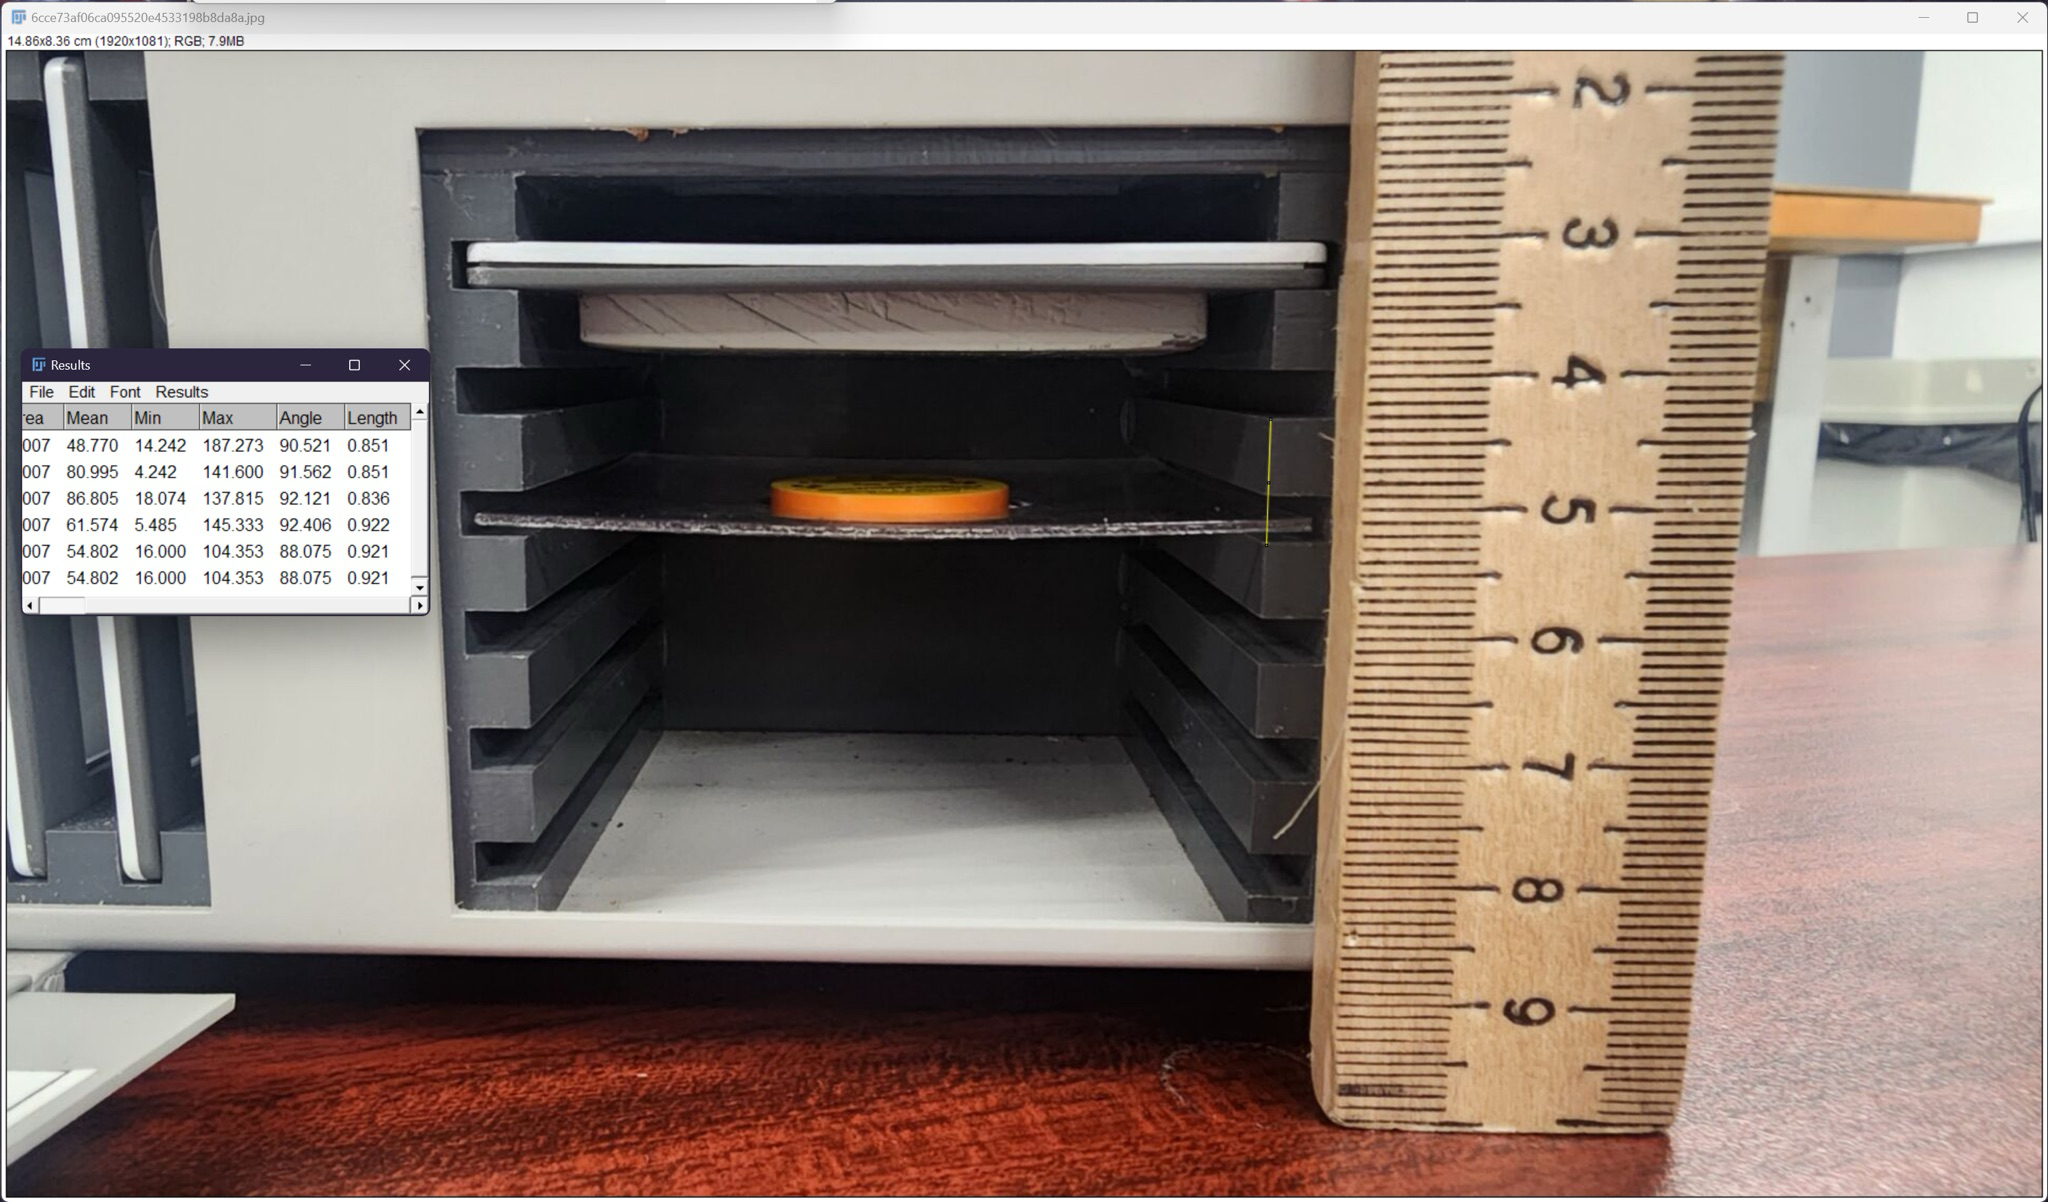
\includegraphics[width=0.82\linewidth]{../assets/experimental_setup_photo.png}
  \caption{Experimental geometry (slot holder and GM counter). The slot separation was measured from this image in Fiji.}
\end{figure}

\section{Data and uncertainty model}
For each configuration we record a gross count rate $N$ and a separate background count rate $B$.
The reported net rate is
\begin{equation}
R \equiv (N-B).
\end{equation}
Assuming Poisson counting statistics for independent counts, the uncertainty in a rate measured over live time $t$ is $\sigma_N \approx \sqrt{N t}/t$.
Where available, we also propagate instrument-reported per-trial rate uncertainties.
For background subtraction (independent measurements), the 1$\sigma$ uncertainty combines in quadrature:
\begin{equation}
\sigma_R = \sqrt{\sigma_N^2 + \sigma_B^2}.
\end{equation}

\section{Analysis and results}\label{sec:analysis}
\subsection{Net rate vs absorber thickness}
We analyzed the gamma-dominated region using the processed dataset in \texttt{data/processed\_points.csv}.
Figure~\ref{fig:nbvsz} shows net rate $(N-B)$ as a function of areal density $Z$ for Slot~2--4.
Ordinary least squares fits for Slot~3 and Slot~4 produce
\begin{align}
(N-B)_{\text{Slot 3}} &= m_3 Z + b_3, & m_3 &= -0.00857, & b_3 &= 263.00,\\
(N-B)_{\text{Slot 4}} &= m_4 Z + b_4, & m_4 &= -0.00595, & b_4 &= 177.95.
\end{align}
The negative slopes quantify the attenuation trend: increasing absorber thickness decreases the detected net rate.

\begin{figure}[H]
  \centering
  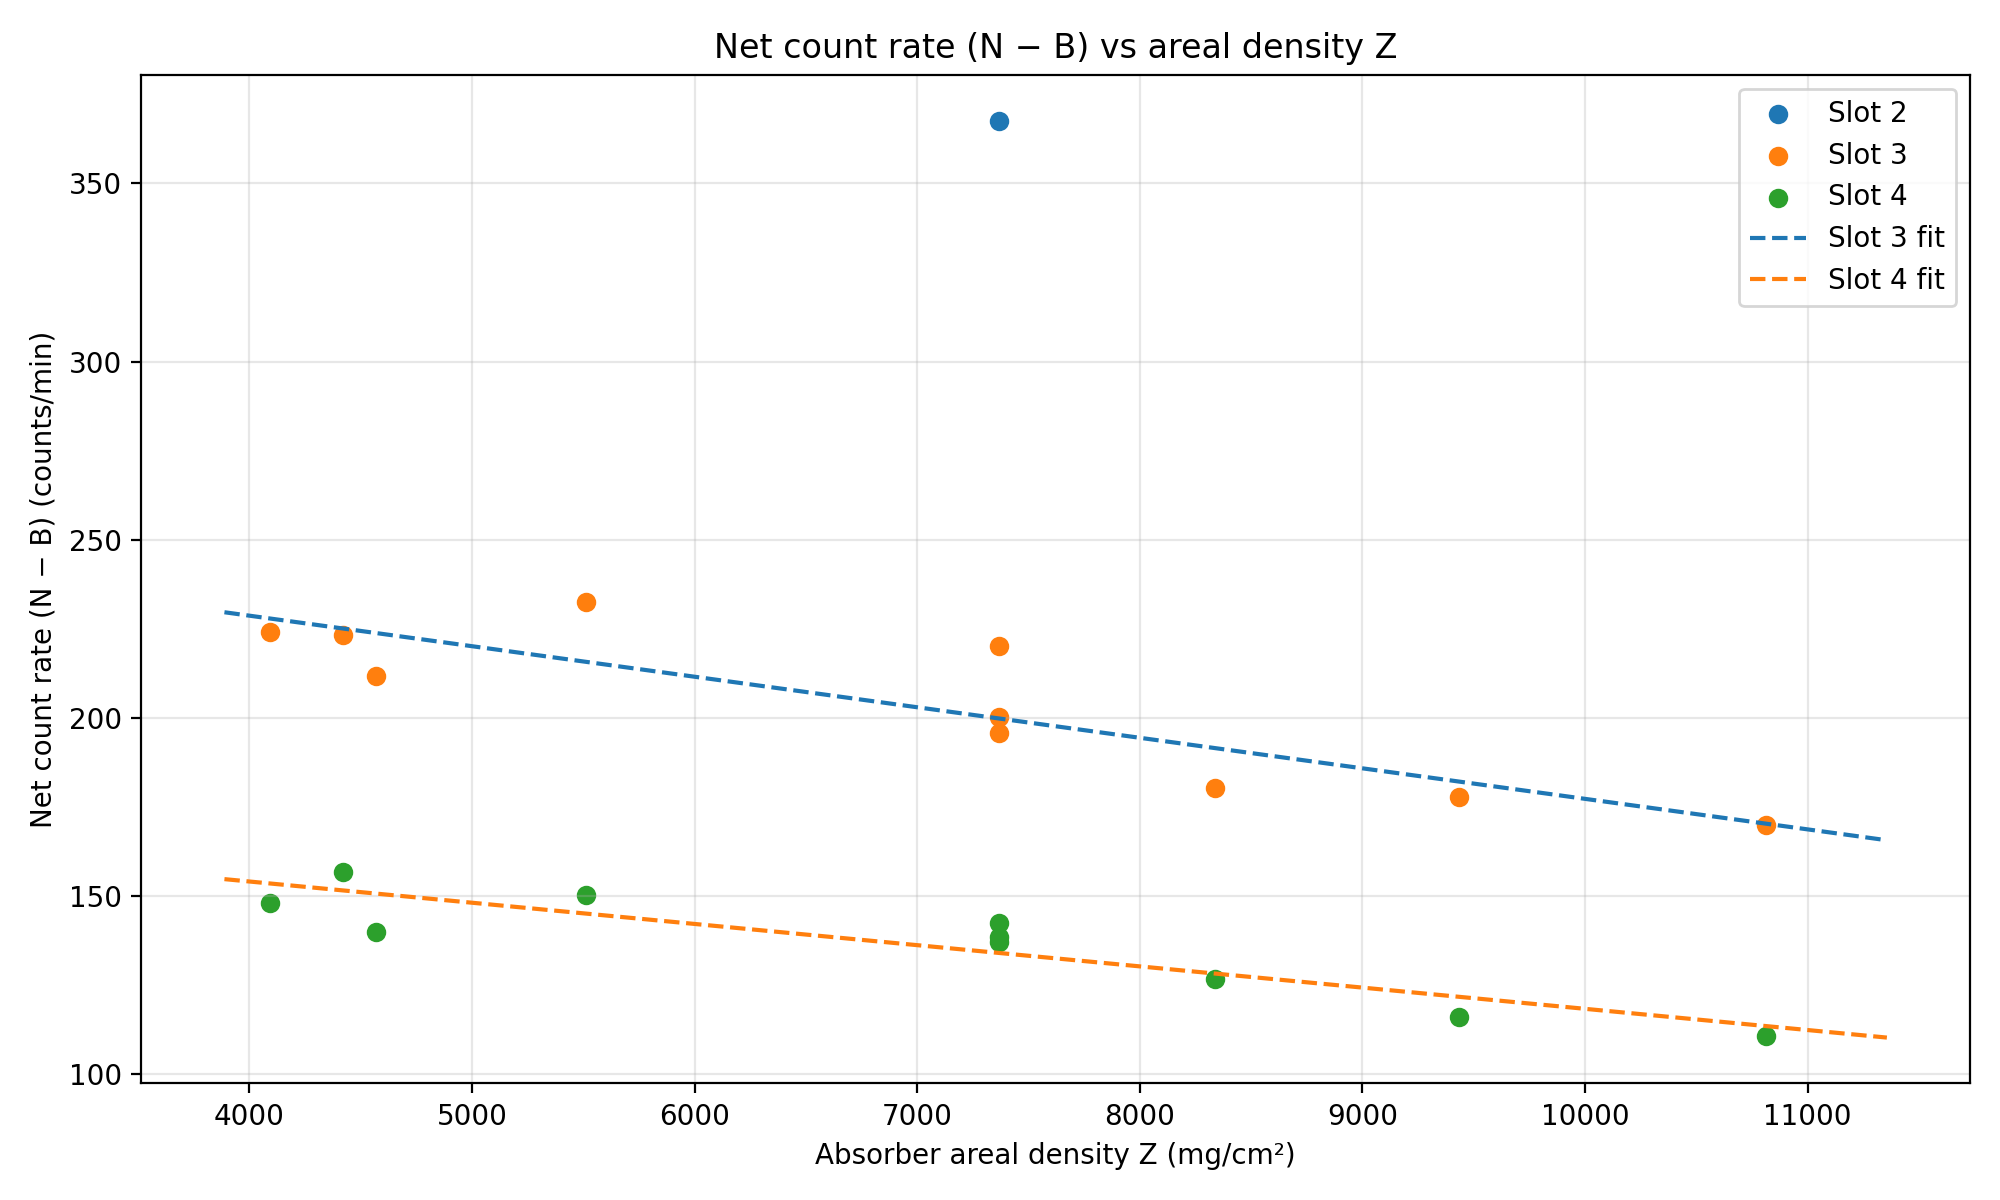
\includegraphics[width=0.92\linewidth]{../figures/nb_vs_z_by_slot.png}
  \caption{Net count rate $(N-B)$ vs absorber areal density $Z$ for different source slots.
  Dashed lines: linear fits for Slot~3 and Slot~4 (gamma-dominated thickness range).}
  \label{fig:nbvsz}
\end{figure}

\subsection{Mapping a source-position change to an equivalent thickness change}
If we require the \emph{same} target net rate $R_\star$ in two geometries, we can invert the fitted relations to obtain the implied thickness:
\begin{equation}
Z(R_\star) = \frac{R_\star - b}{m}.
\end{equation}
For a fixed target $R_\star$, the additional thickness required in Slot~3 relative to Slot~4 is
\begin{equation}
\Delta Z(R_\star) = Z_{3}(R_\star) - Z_{4}(R_\star).
\end{equation}
Over the operating range $R_\star\in[110,150]$\,cpm, $\Delta Z$ is well described by a linear model (Fig.~\ref{fig:deltaz}):
\begin{equation}
\Delta Z \approx 51.38\,R_\star + 781 \quad \text{(\si{mg.cm^{-2}})}.
\end{equation}
Example: for $R_\star=130$\,cpm, $\Delta Z\approx\SI{7.46e3}{mg.cm^{-2}}$.

\begin{figure}[H]
  \centering
  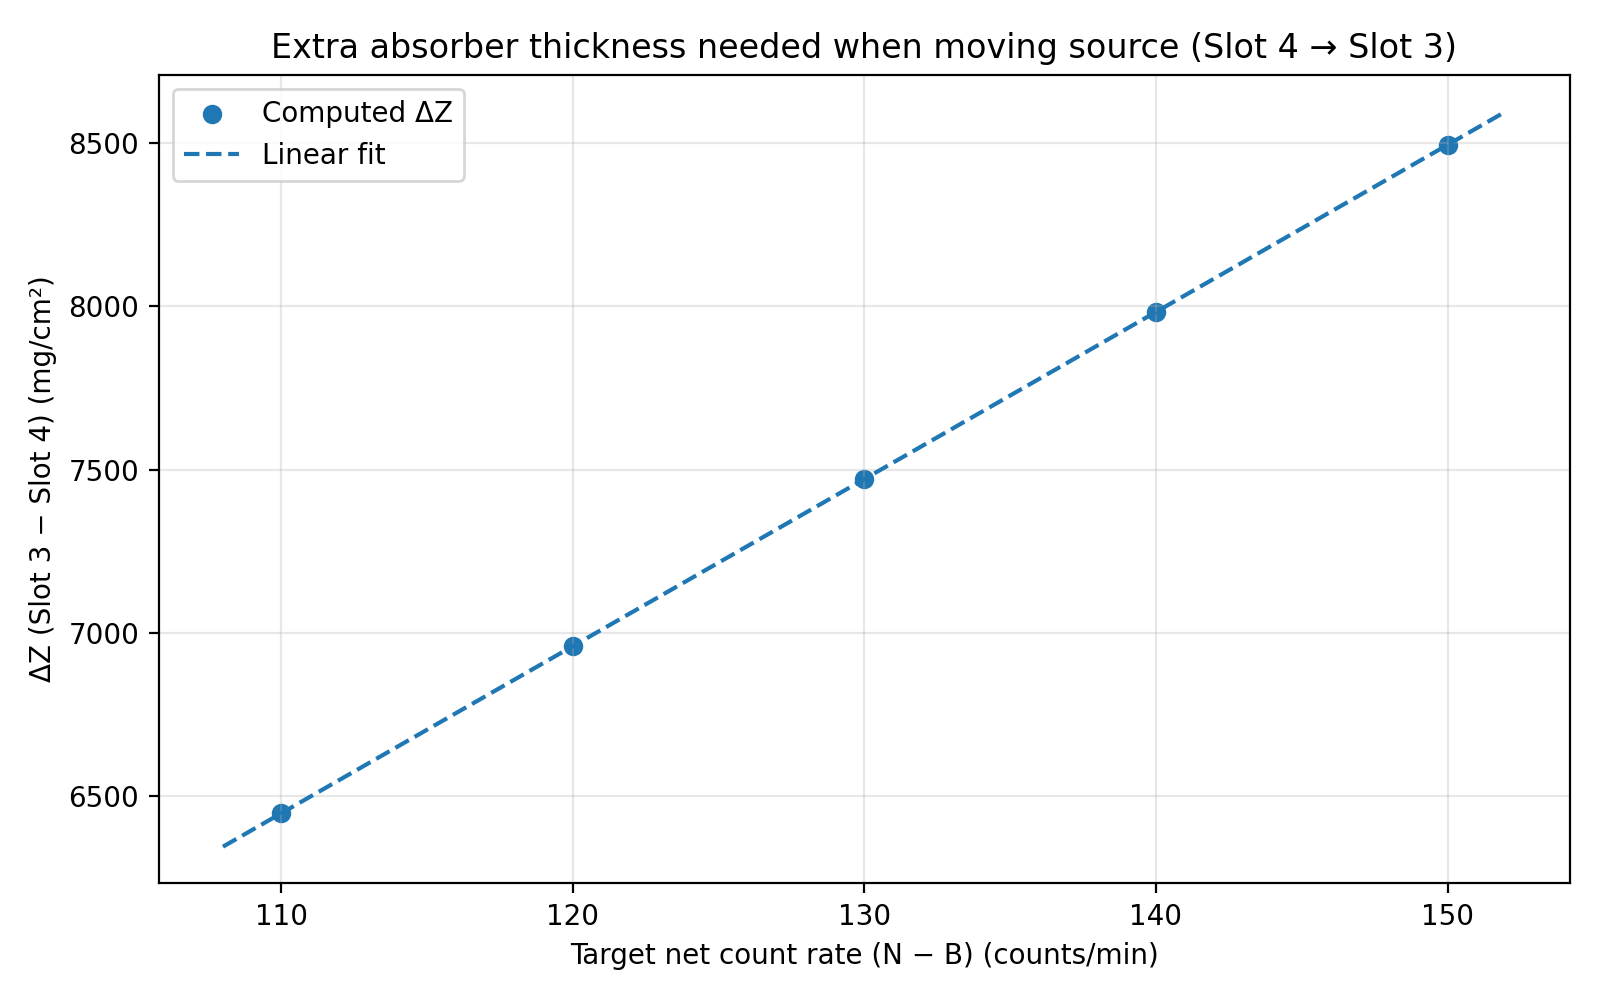
\includegraphics[width=0.86\linewidth]{../figures/deltaZ_vs_nb.png}
  \caption{Equivalent absorber thickness change required when moving the source from Slot~4 to Slot~3 while holding the target net rate fixed.
  Points are computed by inverting the two fitted lines; the dashed line is a linear fit.}
  \label{fig:deltaz}
\end{figure}

\subsection{Control: absorber position}
A control dataset (\texttt{data/raw\_absorber\_position\_test.csv}) measured $(N-B)$ with the same total thickness but with the absorber stack placed in different slots.
The mean net rates are statistically indistinguishable (one-way ANOVA $p=0.70$), supporting the conclusion that absorber position does not measurably affect net rate at fixed $Z$.

\begin{figure}[H]
  \centering
  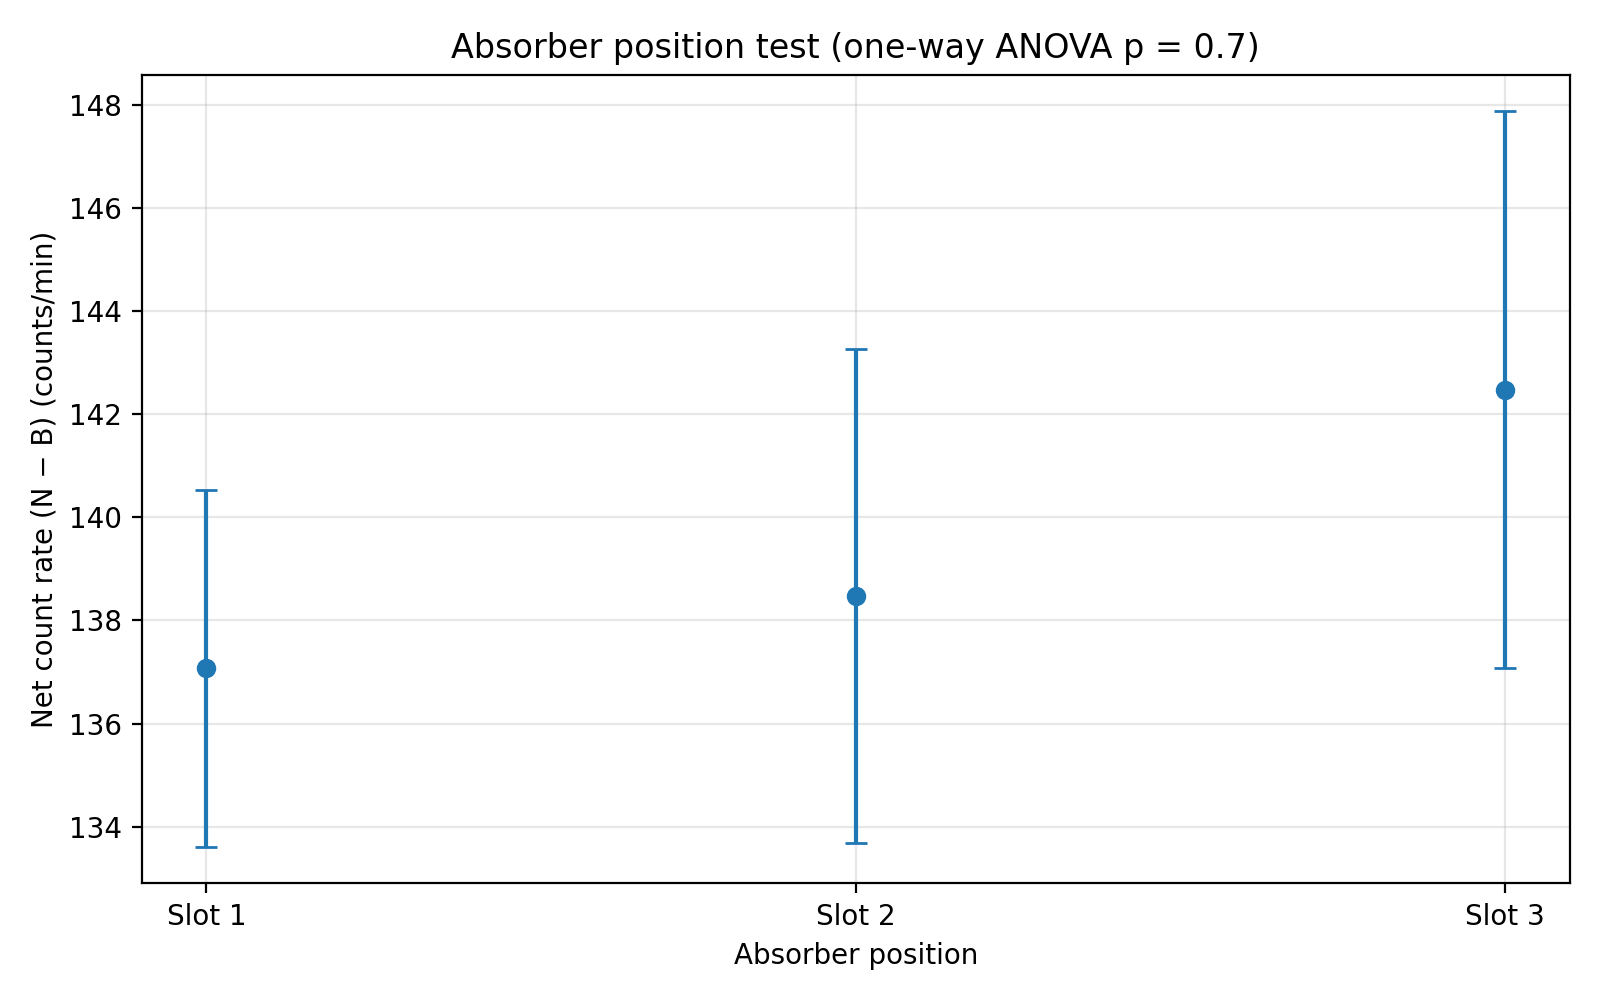
\includegraphics[width=0.70\linewidth]{../figures/absorber_position_net_rates.png}
  \caption{Net rate by absorber position for a fixed thickness $Z=\SI{7367}{mg.cm^{-2}}$ (Slot~4 source).
  Error bars show the standard error of the mean across five trials.}
\end{figure}

\section{Discussion}
The fitted Slot~3 and Slot~4 lines are approximately parallel, implying a systematic shift in net count rate due to geometry rather than a change in attenuation physics.
Because the GM tube samples a finite solid angle, moving the source changes the effective flux incident on the detector, which then maps to a large equivalent thickness change when translated through the attenuation slope.

Key limitations include (i) potential systematic components in the background or rate readout (which would not average down with repeated trials), and (ii) residual beta sensitivity at lower thickness.
A natural extension is to repeat the analysis for additional source slots to map $\Delta Z$ as a function of displacement.

\section{Reproducibility}
All figures and regression coefficients in this report are reproducible from the CSV data and \texttt{src/analyze\_co60.py}.
See \texttt{README.md} for step-by-step instructions.

\appendix
\section{Co-60 decay scheme}
\begin{figure}[H]
  \centering
  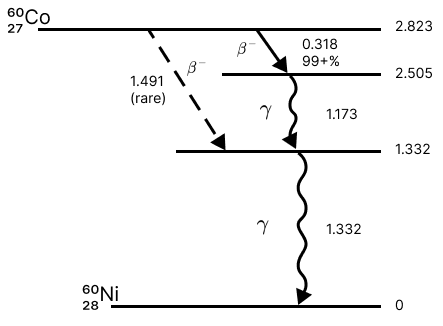
\includegraphics[width=0.55\linewidth]{../assets/co60_decay_scheme.png}
  \caption{Simplified Co-60 decay scheme (beta decay to excited Ni-60 followed by gamma emission).}
\end{figure}

\end{document}
